Close observation of the $N=4$ orbit family, Figure~\ref{fig:monge-orthoptic}, provided invaluable clues with which to generalize $N=3$ invariants to $N>3$ orbits. Namely:

\begin{itemize}
    \item Mittenpunkt: The lines connecting the Tangential Polygon's vertices to the parallelogram midpoints concur at the Ellipse's center.
     \item Null Sum of Cosines: The polygon formed by the four 
     tangency points is a parallelogram therefore the sum of its cosines is zero.
    \item Null Product of Cosines: The Tangential Polygon is a rectangle and therefore the product of its cosines is zero.
   \item Circular Locus: The orthoptic locus is a circle.
\end{itemize}

\subsection{$N>3$ Stationary Point}

Let the Tangential Polygon be the generalization of the Excentral Triangle for $N>3$. The same Affine proof used in Theorem~\ref{thm:olga} and Figure~\ref{fig:mitten} yields:

\begin{theorem}
Given an $N\geq{3}$ orbit family, the point of concurrence of lines drawn from vertices of the tangential polygon through the midpoints of orbit sides is stationary at the center of the Billiard.
\end{theorem}

\noindent This is illustrated in Figure~\ref{fig:gen-mitten} and in   \cite[pl\#13]{dsr_math_intell_playlist}.

\begin{figure}
    \centering
    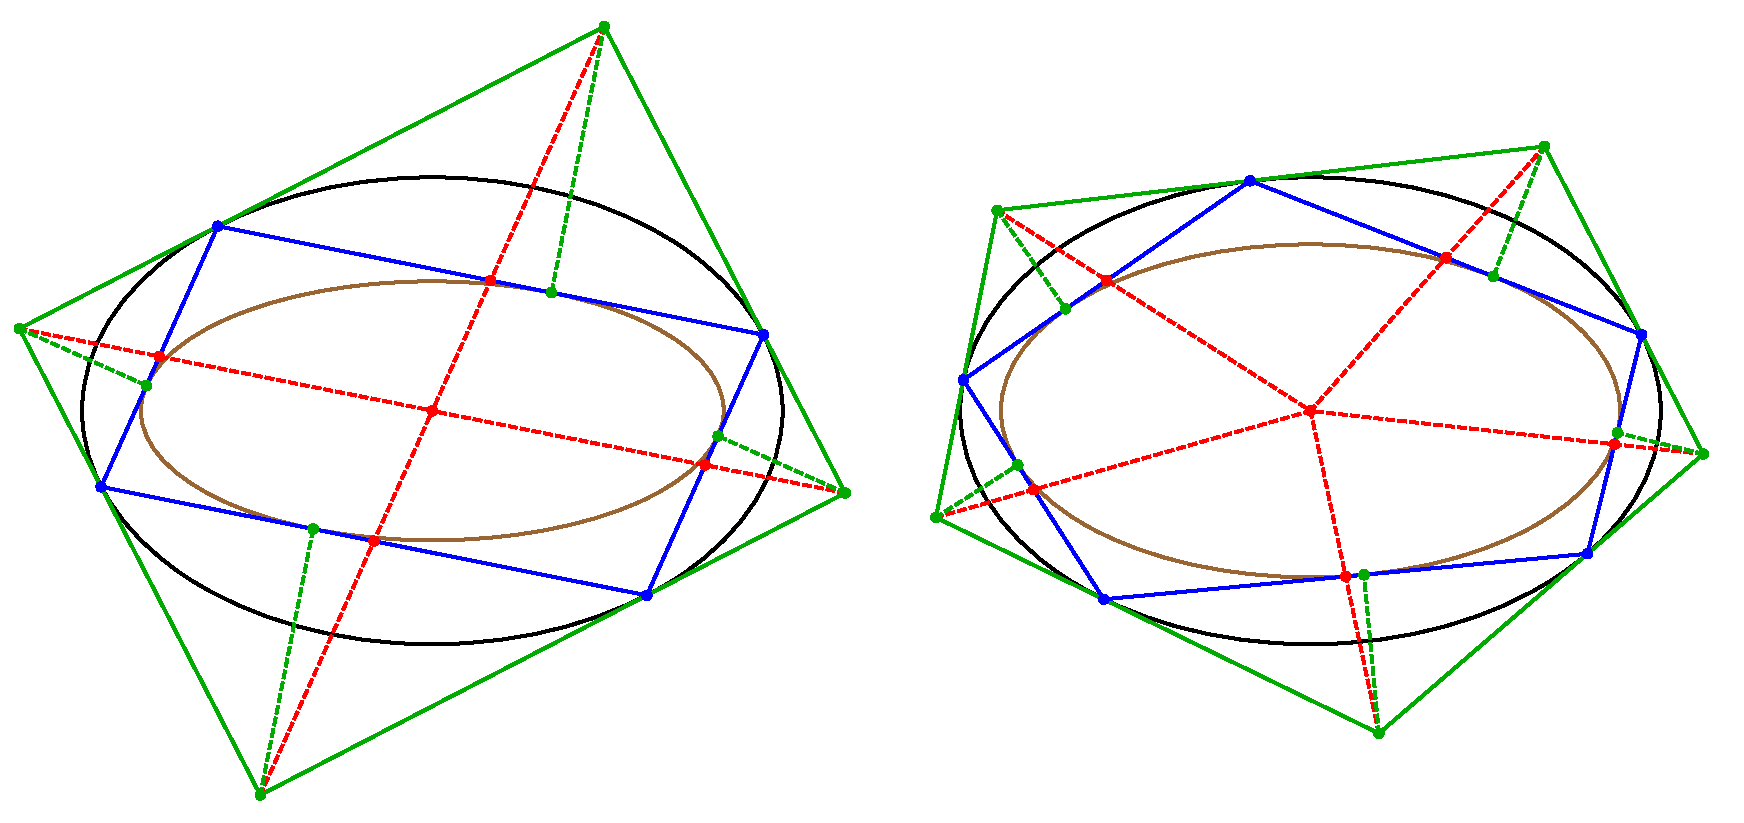
\includegraphics[width=\textwidth]{pics/u0165_extouch.pdf}
    \caption{\textbf{Left}: $N=4$ (resp. \textbf{Right}: $N=5$) orbits shown in blue. The dashed red lines connect vertices of the Tangential (green) to orbit sides' midpoints. Notice they intersect at the center of the Billiard, a type of generalized Mittenpunkt. Also shown are (dashed green) perpendiculars dropped from Tangential Vertices onto orbit sides. Their feet lie on and sweep the Caustic (brown). \href{https://youtu.be/TV2p7fPlYfE}{Video 1}, \href{https://youtu.be/Bpc-MrR2IMc}{Video 2}  \cite[pl\#18,19]{dsr_math_intell_playlist}.}
    \label{fig:gen-mitten}
\end{figure}

\subsection{Generalized Extouchpoints}

Theorem~\ref{thm:extouch} states Extouchpoints are on and sweep the $N=3$ caustic. Analogously, Figure~\ref{fig:gen-mitten}:

\begin{theorem}
The feet of perpendiculars dropped from vertices of the Tangential Polygon onto orbit sides are on the caustic and have the latter as their locus.
\end{theorem}

It turns out the above is a special case of Chasles' Theorem \cite{sergei2016proj}. 

This offers a method to easily ``find'' a point on the caustic which only requires two orbit vertices, alternate to \cite{himmelstrand12} which required the Billiard's foci.

\subsection{$N>3$ Cosine Sum and Product}

The fact that both $N=3$ and $N=4$ conserve cosine sum suggests $N>4$ might as well, and this was first confirmed numerically for $N=5,\ldots,30$ non-intersecting orbits at various Billiard aspect ratios. A proof to this surprising fact has been kindly contributed \cite{sergei19_private_meromorphic}.

\begin{theorem}
The sum of cosines is conserved for non-intersecting orbits, for all $N$. %$\forall{N}$
\label{thm:cosine-sum-meromorphic}
\end{theorem}

\noindent Beyond establishing the sum of cosines was constant, we noticed Equations~\ref{eqn:rR_dominique}~and~\ref{eqn:rR_cos} imply that for $N=3$, $\sum{\cos\theta_i}=\gamma{L}-3$. The appearance of a ``$3$'' suggested we should verify (numerically) if substituting this digit by $N$ would hold for all $N$. Surprisingly this did hold, and a proof soon followed \cite{sergei19_private_cosine_sum_expression}:

\begin{theorem}
For an $N$-periodic orbit, $\sum_{i=1}^{N}{\cos\theta_i}=\gamma{L}-N$.
\label{thm:cosine-sum}
\end{theorem}

\noindent Because all terms $\gamma$, $L$, and $N$ are constant, the above subsumes and is more specific than Theorem~\ref{thm:cosine-sum-meromorphic}. Note that for $N=4$, the sum of cosines is zero and $\gamma{L}=4$, independent of the EB's aspect ratio.

Furthermore, since $\cos\frac{\theta_i}{2}=\frac{\nabla{f_i}.\hat{v}}{||\nabla{f_i}||}=\frac{2\gamma}{||\nabla{f_i}||}$, the following expression for the perimeter $L$ will hold:

\begin{corollary}
\begin{equation}
    L=8\gamma\sum_{i=1}^{N}\frac{1 }{||\nabla{f_i}||^2} \;\cdot
    \label{eqn:perimeter-new}
\end{equation}
\end{corollary}

\noindent Since both $N=3$ and $N=4$ conserve the product of their Excentral/Tangential cosines, we confirmed numerically that $N=5,\ldots,30$ non-intersecting orbits at various aspect ratios also conserve this quantity. It can also be proven that \cite{akopyan19_private_meromorphic}:

\begin{theorem}
The product of cosines for the Tangential Polygon of non-intersecting orbits for {\em any} $N$ is conserved.
\end{theorem}

\subsection{Area Ratio for $N>3$}

For $N=3$ the Excentral-to-Orbit area ratio is conserved, however, we can numerically check this is not the case for $N=4$. Proceeding to $N>4$ we verify that only odd $N$ preserve area ratio, a fact which has been subsequently formally proven \cite{akopyan19_private_meromorphic}.

\begin{theorem}
The ratio of areas between Tangential Polygon and Non-Self-Intersecting Orbit is conserved for all odd $N$.
\end{theorem}

\subsection{$N>4$ Circular Loci}

For the $N=3$ case,  Figure~\ref{fig:cosine_circle_locus}, the locus of the intersection of an Excentral Triangle edge with an alternate edge reflected about the Billiard center is a circle. For $N=4$ we have Monge's Orthoptic Circle. Here is how these two constructions can be unified to $N>4$, Figure~\ref{fig:gen-circ-grid}, \cite[pl\#5]{dsr_math_intell_playlist}:

\begin{theorem}
Let $O$ be the center of the Billiard. The locus of the intersection of an edge of the Tangential Polygon with the reflection of the next tangential edge about $O$ is a circle centered on $O$. Its radius is $r^*=1/\gamma$.
\end{theorem}

\noindent {\bf Proof} \cite{sergei19_private_circles}: Let $\nabla_i$ denote $\nabla{f_i}$ of Equation~\ref{eqn:f}. Consider two consecutive orbit vertices $P_{i}$ and $P_{i+1}$. Momentum conservation (Equation~\ref{eqn:joachim}) implies $\hat{v}.\nabla_i= -\hat{v}.\nabla_{i+1}=2\gamma$. So we have:

\begin{equation}
    \hat{v}.\left(\nabla_i+ \nabla_{i+1}\right)=0\;.
    \label{eqn:sum-nablas}
\end{equation}

\noindent Since $\nabla_i$ (resp. $\nabla_{i+1}$) is normal to the ellipse at $P_{i}$ (resp. $P_{i+1}$), a point $z$ on the tangent line at $P_i$ (resp. $-P_{i+1}$) is given by $z.\nabla_i=2$ (resp. $z.\nabla_{i+1}=-2$). Let $z$ be where both lines intersect, $z.\left(\nabla_i+\nabla_{i+1}\right)=0$. It follows from Equation~\ref{eqn:sum-nablas} that $z$ is parallel to $\hat{v}$. Since $\hat{v}.\nabla_i=2\gamma$ and $z.\nabla_i=2$, we have $z = \hat{v}/\gamma$. That is, $z$ lies on the circle of radius $1/\gamma$.\qed

\begin{figure}[H]
    \centering
        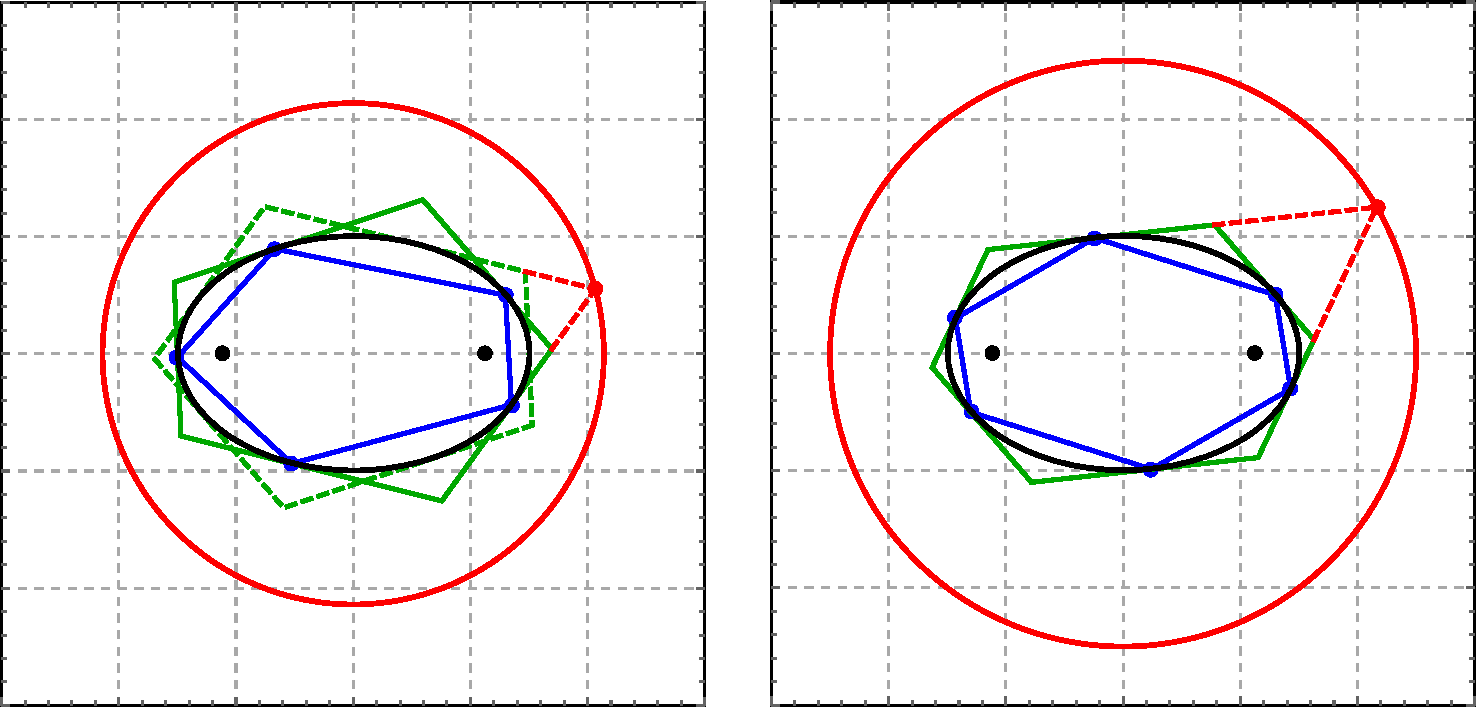
\includegraphics[width=\textwidth]{pics/u0180_circ_grid.pdf}
   % \includegraphics[width=\textwidth,trim={12.75cm 0 0 1cm},clip]{pics/0180_circ_grid_a.pdf}
    \caption{The construction of a circular locus for $N=5,6$.
    % done
    \href{https://youtu.be/dINE4aH1cvk}{Video 1},
    % done
    \href{https://youtu.be/EFeINGIDFrg}{Video 2} \cite[pl\#20,21]{dsr_math_intell_playlist}}
    \label{fig:gen-circ-grid}
\end{figure}
